%%%%%%%%%%%%%%%%%%%%%%%%%%%%%%%%%%%%%%%%%%%%%%%%%%%%%%%%%%%%%%%%%%%%%%%%
%                                                                      %
% GLE - Graphics Layout Engine <http://www.gle-graphics.org/>          %
%                                                                      %
% Modified BSD License                                                 %
%                                                                      %
% Copyright (C) 2009 GLE.                                              %
%                                                                      %
% Redistribution and use in source and binary forms, with or without   %
% modification, are permitted provided that the following conditions   %
% are met:                                                             %
%                                                                      %
%    1. Redistributions of source code must retain the above copyright %
% notice, this list of conditions and the following disclaimer.        %
%                                                                      %
%    2. Redistributions in binary form must reproduce the above        %
% copyright notice, this list of conditions and the following          %
% disclaimer in the documentation and/or other materials provided with %
% the distribution.                                                    %
%                                                                      %
%    3. The name of the author may not be used to endorse or promote   %
% products derived from this software without specific prior written   %
% permission.                                                          %
%                                                                      %
% THIS SOFTWARE IS PROVIDED BY THE AUTHOR "AS IS" AND ANY EXPRESS OR   %
% IMPLIED WARRANTIES, INCLUDING, BUT NOT LIMITED TO, THE IMPLIED       %
% WARRANTIES OF MERCHANTABILITY AND FITNESS FOR A PARTICULAR PURPOSE   %
% ARE DISCLAIMED. IN NO EVENT SHALL THE AUTHOR BE LIABLE FOR ANY       %
% DIRECT, INDIRECT, INCIDENTAL, SPECIAL, EXEMPLARY, OR CONSEQUENTIAL   %
% DAMAGES (INCLUDING, BUT NOT LIMITED TO, PROCUREMENT OF SUBSTITUTE    %
% GOODS OR SERVICES; LOSS OF USE, DATA, OR PROFITS; OR BUSINESS        %
% INTERRUPTION) HOWEVER CAUSED AND ON ANY THEORY OF LIABILITY, WHETHER %
% IN CONTRACT, STRICT LIABILITY, OR TORT (INCLUDING NEGLIGENCE OR      %
% OTHERWISE) ARISING IN ANY WAY OUT OF THE USE OF THIS SOFTWARE, EVEN  %
% IF ADVISED OF THE POSSIBILITY OF SUCH DAMAGE.                        %
%                                                                      %
%%%%%%%%%%%%%%%%%%%%%%%%%%%%%%%%%%%%%%%%%%%%%%%%%%%%%%%%%%%%%%%%%%%%%%%%

\chapter{QGLE: GLE's Graphical User Interface}
\index{QGLE}\label{QGLE:chap}

QGLE is the graphical user interface (GUI) to GLE. A screenshot of QGLE with some of its dialogs appears in Fig.~\ref{fig:qgle}.

\begin{figure}
\resizebox{\textwidth}{!}{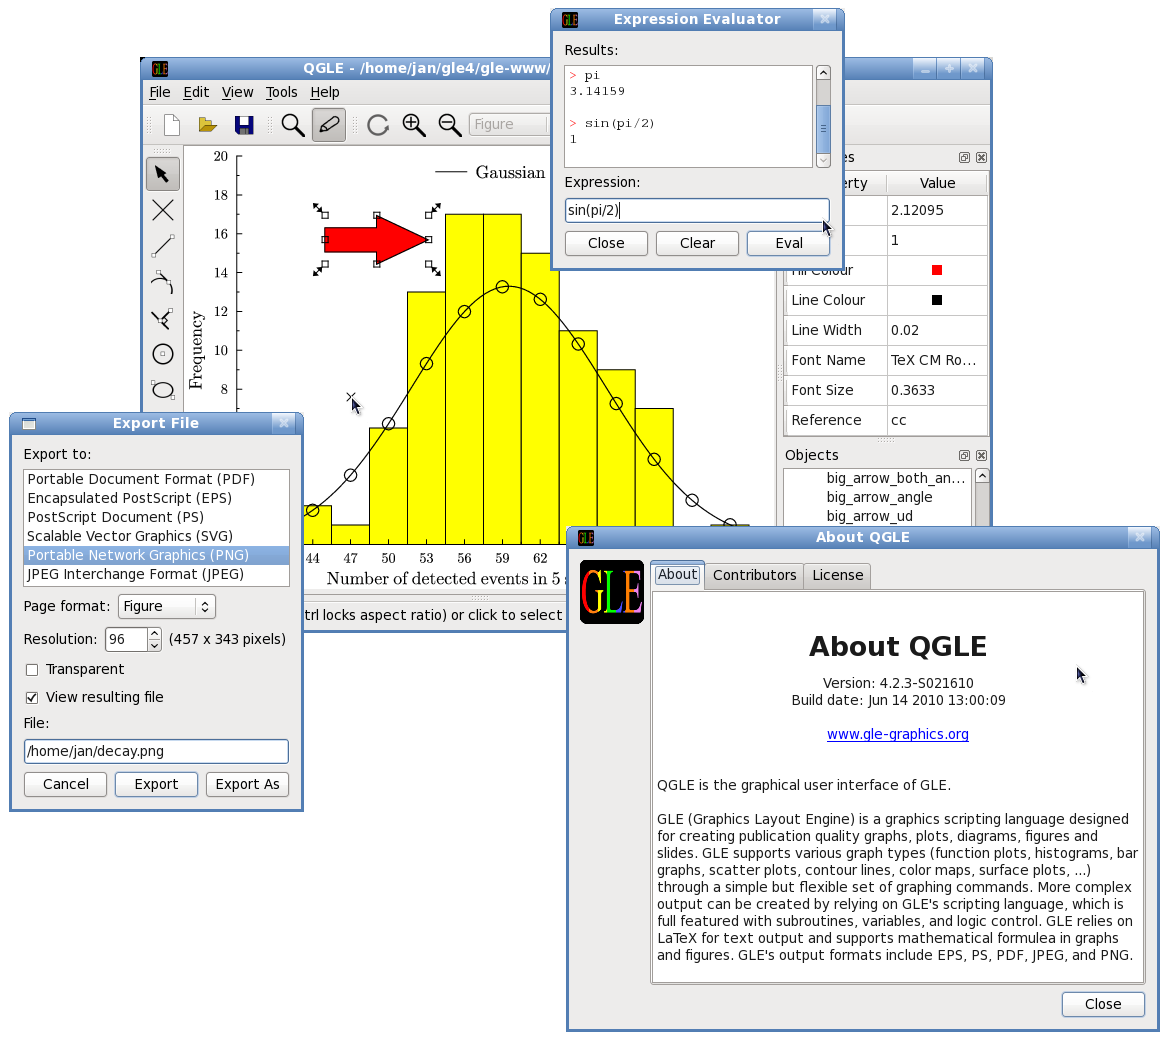
\includegraphics{qgle/screenshot/qgle-windows1.png}}
\caption{\label{fig:qgle}A screenshot of QGLE.}
\end{figure}

The current GUI contains a preview window that can receive messages from GLE and display the resulting EPS file. In addition, it can open GLE and EPS files directly (using Ghostscript and GLE).  It has the capability to add and edit simple objects, such as, lines, circles, arcs (snapping to a grid if required), and complex object blocks (defined with begin/end object). It can also alter various properties of the objects, such as, line width, and color. The perpendicular line and tangential line commands can be used to produce a line starting perpendicular or tangential to an existing object. OSnap can be used for the end point of a line.

\vspace{0.5cm}
When drawing objects, hit the escape key to cancel.  The pointer tool can be used to select objects and they can be deleted using the 'del' key or moved/scaled. Shift can be used to select multiple objects.

\vspace{0.5cm}
Keyboard shortcuts include:

\begin{tabular}{l|l}
F1 & Open the GLE manual \\
F3 & Toggle object snap \\
F6 & Toggle coordinate display \\
F7  & Toggle grid visibility \\
F8  & Toggle orthographic snap \\
F9  & Toggle grid snap \\
F10 & Toggle polar snap \\
'-' & Zoom in \\
'=' & Zoom out \\
\end{tabular}
